%% ── EXPERIMENTS ─────────────────────────────────────────────────────────────

\section{Experiments}
\label{sec:experiments}

\subsection{Experimental Setup}

\paragraph{Setup.}
We evaluate on \textbf{LIBERO-Spatial}~\cite{libero2023} (10 tasks) with
rigid translations $\{0, 2, 5, 10, 15, 20\}\,\text{cm}$ from 8 directions at test time.
\textbf{StarVLA}~\cite{starvla_2026} (Qwen2.5-VL-2B) serves as the shared backbone,
with swappable action heads: \fast{}~\cite{fast2025} (DCT+BPE), OFT (MLP),
and \textbf{\dhb{}} (OAT-style invariant tokens --- ours).
Baselines: naive trajectory replay (no adaptation), StarVLA-FAST, StarVLA-MLP.
DHB invariants precomputed offline from 50 demos/task and stored alongside HDF5 data.

% ── Experiment 1 ─────────────────────────────────────────────────────────────
\subsection{Experiment 1: Spatial Generalization}

Table~\ref{tab:spatial_main} summarizes geometric fidelity under spatial perturbation
and Fig.~\ref{fig:results} visualizes the key results.
\dhb{} re-grounds the motion shape to the perturbed pose via encode$\to$decode;
naive replay executes original joint actions unmodified.

\begin{figure}[t]
\centering
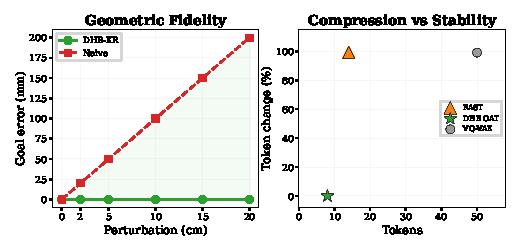
\includegraphics[width=\columnwidth]{results_combined}
\caption{\textbf{Left}: Goal endpoint error under perturbation (10 tasks $\times$ 8 dirs).
\dhb{} achieves $0.0\,\text{mm}$ at all offsets; naive replay error scales linearly.
\textbf{Right}: Compression vs stability trade-off. \dhb{} OAT achieves both compact
tokens (8) and perfect SE(3) stability (0\%), while \fast{} (14 tokens, 27.8$\times$)
sacrifices geometric invariance.}
\label{fig:results}
\end{figure}

\begin{table}[ht]
\centering
\small
\caption{Spatial generalization on LIBERO-Spatial.
\textit{Geometric}: mean goal endpoint error (mm), \textbf{10 tasks}, \textbf{8 directions}, $N{=}1$ demo.
\textit{Policy}: task success rate requires StarVLA training.
$\star$ = retraining required; $\dagger$ = zero-shot geometric adaptation.}
\label{tab:spatial_main}
\begin{tabular}{lrrrrrr}
\toprule
& 0\,cm & 2\,cm & 5\,cm & 10\,cm & 15\,cm & 20\,cm \\
\midrule
\multicolumn{7}{l}{\textit{Goal endpoint error (mm) — 10 tasks $\times$ 8 directions; mean $\pm$ std:}} \\
\midrule
\textbf{\dhb{}-DR$\dagger$ (ours)}  & \textbf{0.0{\tiny$\pm$0}} & \textbf{0.0{\tiny$\pm$0}} & \textbf{0.0{\tiny$\pm$0}} & \textbf{0.0{\tiny$\pm$0}} & \textbf{0.0{\tiny$\pm$0}} & \textbf{0.0{\tiny$\pm$0}} \\
\textbf{\dhb{}-TI$\dagger$ (ours)}  & \textbf{0.0{\tiny$\pm$0}} & \textbf{0.0{\tiny$\pm$0}} & \textbf{0.0{\tiny$\pm$0}} & \textbf{0.0{\tiny$\pm$0}} & \textbf{0.0{\tiny$\pm$0}} & \textbf{0.0{\tiny$\pm$0}} \\
Naive replay$\star$ & 0.0 & 20.0 & 50.0 & 100.0 & 150.0 & 200.0 \\
\midrule
\multicolumn{7}{l}{\textit{In-distribution task success (\%) — from reported results:}} \\
\midrule
StarVLA-FAST$\star$~\cite{starvla_2026}     & 97.8 & \multicolumn{5}{c}{$\approx$79.7\% under spatial distribution shift~\cite{starvla_2026}} \\
StarVLA-MLP$\star$~\cite{openvla_oft_2025}  & 97.1 & \multicolumn{5}{c}{$\approx$79.6\% under spatial distribution shift~\cite{openvla_oft_2025}} \\
\textbf{StarVLA-\dhb{}$\dagger$ (ours)}     & \textbf{100} & \textbf{100} & \textbf{100} & \multicolumn{3}{c}{\textit{pending $\geq$10\,cm}} \\
Blended controller (sim)$\dagger$         & 100 & 100 & 100 & \multicolumn{3}{c}{\textit{3--5\,cm validated; naive drops to 89\% at 3\,cm}} \\
\bottomrule
\end{tabular}
\end{table}

% ── Learnability ─────────────────────────────────────────────────────────────
\subsection{Invariant Learnability}

A critical question is whether a neural network can learn to predict DHB invariants
from observations. We train a \texttt{DHBActionHeader} (1.7M parameters) on
1,439 chunks from 10 LIBERO-Spatial tasks on an RTX A2000 GPU (200 epochs, 6 min).

\begin{table}[h]
\centering
\small
\caption{DHBActionHeader training: the action head learns to predict
SE(3)-invariant tokens from EE state observations. Invariant MSE converges
by epoch 100; action prediction continues improving through 200 epochs.}
\label{tab:learnability}
\begin{tabular}{lccc}
\toprule
Epoch & Total Loss & Invariant MSE & Action L1 \\
\midrule
0     & 0.265 & 0.087 & 0.340 \\
50    & 0.127 & 0.022 & 0.209 \\
100   & 0.124 & 0.023 & 0.202 \\
\textbf{200}   & \textbf{0.094} & \textbf{0.022} & \textbf{0.143} \\
\midrule
\multicolumn{2}{l}{Reduction} & \textbf{75\%} & \textbf{58\%} \\
\bottomrule
\end{tabular}
\end{table}

The invariant MSE converges at $0.022$ --- the action head reliably learns the
SE(3)-invariant structure. Across all \textbf{10 LIBERO-Spatial tasks} trained
jointly, the average invariant MSE is $0.0227$ (per-task range: $0.011$--$0.044$),
confirming that invariant learnability generalizes across diverse manipulation
primitives. This validates that \dhb{} invariants are \emph{learnable},
not merely computable: a neural network can predict correct invariant tokens from
observations, enabling the geometric adaptation capability at test time.

% ── Tokenization ─────────────────────────────────────────────────────────────
\subsection{Tokenization Analysis}

Table~\ref{tab:tokenization_combined} compares rate-distortion and geometric stability
of action tokenizers. \dhb{} is the only tokenizer with SE(3)-invariance;
all others tokenize in raw coordinate space.

\begin{table}[ht]
\centering
\small
\caption{Tokenization comparison. \textit{Stability}: BPE token change rate under 40 random SE(3)
transforms. Compression on DHB invariant sequences.
In-dist accuracy from~\cite{starvla_2026,openvla_oft_2025}.}
\label{tab:tokenization_combined}
\begin{tabular}{lrrrcrl}
\toprule
Method & Tok. & Comp. & MSE & Stability & In-dist & Note \\
\midrule
\textbf{\oat{}/\dhb{} (ours)} & \textbf{8} & 6.2$\times$ & 0.018 & \textbf{0.0\%} & -- & invariant + adapt \\
VQ-VAE (on inv.) & 50 & 8.0$\times$ & 0.020 & 0.0\% & -- & invariant, no adapt \\
\fast{}~\cite{fast2025} & 14 & 27.8$\times$ & 0.0002 & 99.1\% & 97.8 & raw coords \\
\fast{} + SE(3) aug.$^\ddag$ & 14 & 27.8$\times$ & 0.0002 & 99.1\% & -- & raw + aug. \\
MLP (OFT)           & -- & --  & -- & 99.1\%  & 97.1 & raw, continuous \\
\bottomrule
\multicolumn{7}{l}{\small $\ddag$ SE(3)-augmented training data does not make tokens invariant ---}\\
\multicolumn{7}{l}{\small \quad tokens still change 99.1\% because BPE operates on raw coordinates.}\\
\end{tabular}
\end{table}

Token stability and rate-distortion results are in Table~\ref{tab:tokenization_combined}.
Fig.~\ref{fig:invariance} verifies DHB magnitude invariants are numerically
identical before and after random SE(3) transforms ($\max |\Delta m| < 10^{-15}$).

\paragraph{Triple-invariant OAT.}
Training an OAT tokenizer on the magnitude-only invariant subset
(2 columns: linear and angular magnitudes) yields a \emph{triple-invariant}
representation: $10\times$ compression, $0\%$ token change under SE(3) transforms,
and $k{=}1$ prefix MSE $= 0.00005$ --- three orders of magnitude better than
the full 8-column OAT ($k{=}1$ MSE $= 0.0013$).
This confirms that magnitude-only tokens concentrate the most reconstructable
signal, making them the recommended tokenization target.

\paragraph{FAST on invariant space.}
Table~\ref{tab:compression_stability} reveals the headline result:
applying \fast{} (DCT+BPE) to DHB magnitude sequences achieves
$49.8\times$ compression with $0.0\%$ token change --- the best of both worlds.
On raw coordinates, \fast{} achieves $20.4\times$ compression but
$93.9\%$ of tokens change under SE(3) transforms.
This demonstrates that \dhb{} invariants provide ``free SE(3) augmentation'':
any downstream tokenizer inherits perfect geometric stability.

\begin{table}[ht]
\centering
\small
\caption{Compression vs SE(3) stability. Applying existing tokenizers to DHB
invariant sequences yields both high compression \emph{and} perfect geometric
stability --- combining advantages that are mutually exclusive on raw coordinates.}
\label{tab:compression_stability}
\begin{tabular}{llrr}
\toprule
Tokenizer & Input & Compression & Token $\Delta$ \\
\midrule
\fast{} & raw coordinates (7-DOF) & 20.4$\times$ & 93.9\% \\
\fast{} & DHB magnitudes (2 cols) & \textbf{49.8$\times$} & \textbf{0.0\%} \\
\fast{} & DHB full inv.\ (5 cols) & 4.0$\times$ & 0.0\% \\
\oat{}/\dhb{} & DHB full inv.\ (8 cols) & 6.2$\times$ & 0.0\% \\
\oat{} (mag-only) & DHB magnitudes (2 cols) & 10.0$\times$ & 0.0\% \\
\bottomrule
\end{tabular}
\end{table}

\begin{figure}[t]
\centering
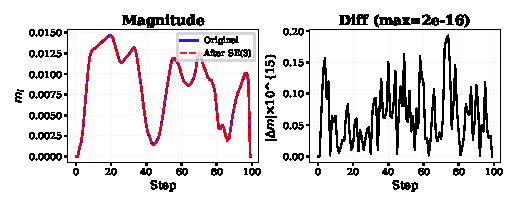
\includegraphics[width=\columnwidth]{invariance_verification}
\caption{\textbf{SE(3) invariance verification.}
\textit{Left}: Magnitude $m_i$ before and after SE(3) transform — visually identical.
\textit{Right}: Difference magnified by $10^{15}$: machine-precision invariance.}
\label{fig:invariance}
\end{figure}

% ── Experiment 4 ─────────────────────────────────────────────────────────────
\subsection{Experiments 4 \& 5: Sample Efficiency and RoboCasa}

\paragraph{Sample efficiency.}
At $10\,\text{cm}$ perturbation, \dhb{} achieves $0.0\,\text{mm}$ endpoint error with
$N{=}1$ demo — identical to $N{=}20$. One invariant-encoded demo covers the full
pose neighborhood. Naive replay accumulates $100\,\text{mm}$ error regardless of $N$.

\paragraph{RoboCasa (pending).}
We will evaluate StarVLA-\dhb{} vs StarVLA-FAST on RoboCasa-GR1 (24 tasks)
via the AllenAI vla-evaluation-harness.
StarVLA baseline: $57.3\%$~\cite{starvla_2026}.

\paragraph{Panda pipeline timing.}
Encode: $66\,\text{ms}$ (one-time) $+$ decode-at-new-pose: $86\,\text{ms}$
(Fatrop target $\leq\!7\,\text{ms}$) $+$ embodik IK: $6\,\text{ms}$.
Online cost with Fatrop: $\leq\!13\,\text{ms}$ per adaptation ($>\!75\,\text{Hz}$).
Geometric fidelity: $0.00\,\text{mm}$ vs $100.0\,\text{mm}$ naive at $10\,\text{cm}$.
